\documentclass{article}
\usepackage{setspace}
\usepackage{graphicx}
\usepackage{subfigure}
\usepackage{amsmath}
\usepackage{pythonhighlight}
\usepackage{longtable}
\usepackage{booktabs}
\usepackage{geometry}
\usepackage{xcolor}
\usepackage{caption}
\usepackage{amsfonts,amssymb}
\usepackage{multirow}
\usepackage{subfigure}
\usepackage{braket}
\usepackage{listings}
\geometry{a4paper,scale=0.8}

\begin{document}
	\begin{titlepage}
		\begin{center}
			\vspace*{1cm}
			\Large{\textbf{DSA5104}}\\
			\Large{\textbf{Principles of Data Management and Retrieval}}\\
			\vspace{1cm}
			\small
			National University of Singapore\\
			Data Science and Machine Learning Department\\
			\today \\
			\vfill
			%School of Mathematics and Science\\
			%Soochow University \\
			%\line(1,0){400}\\[1mm]
			\LARGE{\textbf{Airbnb Dataset Report}}\\[5mm]
			%\Large{\textbf{-The Research on Students' Admission-}}\\[1mm]
			%\line(1,0){400}
			\vfill
			\small
			Wang Jiangyi, A0236307J\\
			Yang Sizhe, A0236299N\\
			Song Mingyue, A0251125U\\
			Lou Xinyun, A0251245M\\
		\end{center}
	\end{titlepage}
	\section{Framework of Report}
	According to the tasks in the project page, we can divide the whole report into seven parts, each of which corresponds to one task:
	\vspace{5pt}
	\\
	1. \textbf{Exploration Data Analysis}. Here, we aim to \textbf{dive into the details} of dataset so that we can deeply understand the resources we have. Beyond that, we also \textbf{dig some interesting patterns} behind data itself. This can gives us some insights and discovers problems from data.
	\\
	2.\textbf{ Data Cleaning}. Based on the EDA we have done, we try to \textbf{fix issues within data}, including the null values and the data types issue. We will also take multi-language issue into consideration.
	\\
	3. \textbf{Data Generation}. We want to \textbf{enrich our data resources} from this part. We will generate transaction records from review records.
	\\
	4. \textbf{Requirement Analysis}. Before designing the database, we do the Requirement Analysis in a \textbf{comprehensive manner}. In our report, we will conduct the analysis from, \textbf{naive user level} and \textbf{host level}. Based on this, we can further write queries to fulfill these requirements.
	\\
	5. \textbf{Relational Database Storage}. According to the pipeline of designing relational database (ER diagram - schema diagram - schema refinement), we will transform \textbf{cleaning data and generating data} into\textit{ \textbf{Mysql DBMS}.}
	\\
	6. \textbf{Non-relational Database Storage}. To take full advantages of  non-relational database, we \textbf{conduct an ad-hoc schema design for it} to store the data in \textbf{\textit{MongoDB DBMS}}.
	\\
	7. \textbf{Query Answer}. In this part, for 2 different database systems, we give the queries based on our requirement anlalysis \textbf{respectively}. Besides, we will \textbf{create index in some attributes} to accelarate the data retrieving process and report the response time and \textbf{comparison will be conducted}.
	\section{Exploration Data Analysis}
	Before showing the data exploration result, we briefly discuss the \textbf{benefits of EDA}. 
	\vspace{3pt}
	\\
	\textbf{Firstly}, in order to transform all the data into database, it is necessary for us to dive into some details of data itself. This can give us some better sense of the dataset, \textbf{which will be beneficial to the following database design process}. Moreover, we can also \textbf{gain insights} from this process, which can \textbf{help business side in application}.
	\vspace{3pt}
	\\
	\textbf{Secondly}, when going through the dataset in details, you can easily find some issues within the data. For example, when checking the boxplot of some attributes, then those outliers can be easily detected if existed. \textbf{This will give us some help with respect to data cleaning process}.
	\vspace{3pt}
	\\
	\textbf{Lastly}, from the real-life application perspective, \textbf{doing EDA carefully will throw some problems} to us. That is, we may discover some abnormal patterns from the data. After observing that, we can \textbf{pose those problems to the technical side and business side} and require their help to solve the problems, which can bring many benefits to the company.
	\vspace{3pt}
	\\
	In our report, we focus on \textbf{the insights} and \textbf{the problems} (\textbf{1} and \textbf{3}) during data exploration process. The exploration details for each dataset can be shown as follows:
	\subsection{calendar}
	In the beginning, we \textbf{make some description} to the 'calendar' dataset. 
	\vspace{3pt}
	\\
	1. The 'calendar' dataset is created around July, 2022 (\textbf{same as other 4 datasets}). 
	\\
	2. This dataset is about, \textbf{for each listing rental}, its price, availability and order requirement information \textbf{within the following 1 year time window}.
	\vspace{3pt}
	\\
	Then, we start to show the discovery result and some intuitive comments:
	\subsubsection{Average price across months}
	Here, we visualize the \textbf{\textit{average price} for all rental in different months}. This can give us some sense about the price changing trend corresponding to different period of year. The visualization result can be shown in Figure \ref{fig:001}:
	\newpage
	\begin{figure}[h]
		\centering
		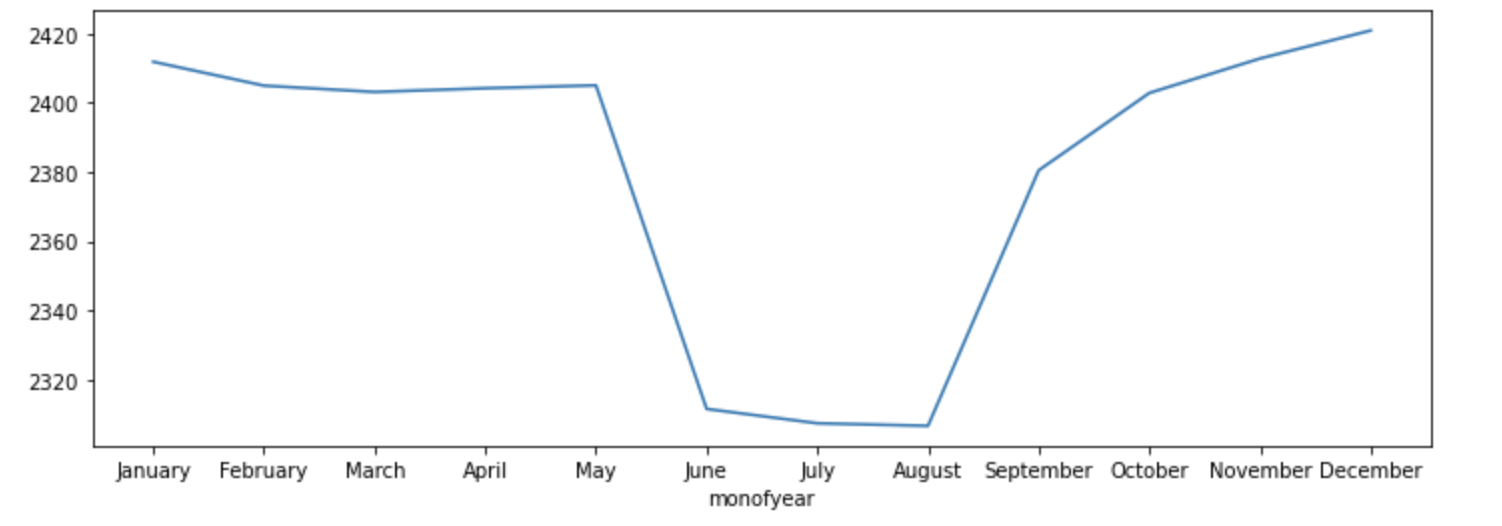
\includegraphics[width=.52\textheight]{avg_price_month.png}
		\caption{Average Price in Different Months}
		\label{fig:001}
	\end{figure}
	\noindent
	\textbf{There is a sharp slope in June, July and August}, which is an abnormal observation. 
	\vspace{3pt}
	\\
	After searching for some information, \textbf{one reasonable reason} is: on June, July and August, students are on their holiday. Therefore, when they plan a trip to some other countries and use Airbnb app to find rentals, they are likely to prefer long-term rental. In this case, the host can give some discounts to them compared with short-term rental.
	\subsubsection{Average price across weekdays}
	Here, we visualize the\textbf{ \textit{average price} in different weekdays}, i.e., from Monday to Sunday. The visualization result can be shown in Figure \ref{fig:002}:
	\begin{figure}[h]
		\centering
		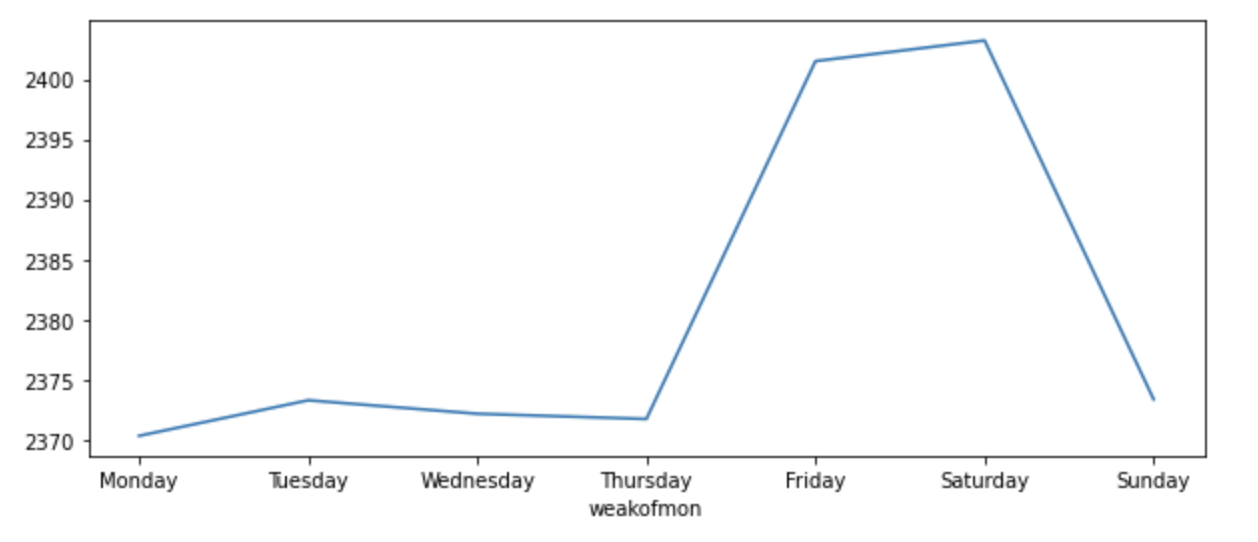
\includegraphics[width=.43\textheight]{avg_price_weekday.png}
		\caption{Average Price in Different Weekdays}
		\label{fig:002}
	\end{figure}
	\\
	The pattern here is close to our intuition: People are busy from Monday to Thursday, and when they want to have a short-term rest, they prefer to choose Friday or Saturday.
	\subsubsection{Busy rate in one year}
	We calculate the \textbf{\textit{busy rate} for all rentals} and do the visualization. The result is shown in Figure \ref{fig:003}:
	\begin{figure}[h]
		\centering
		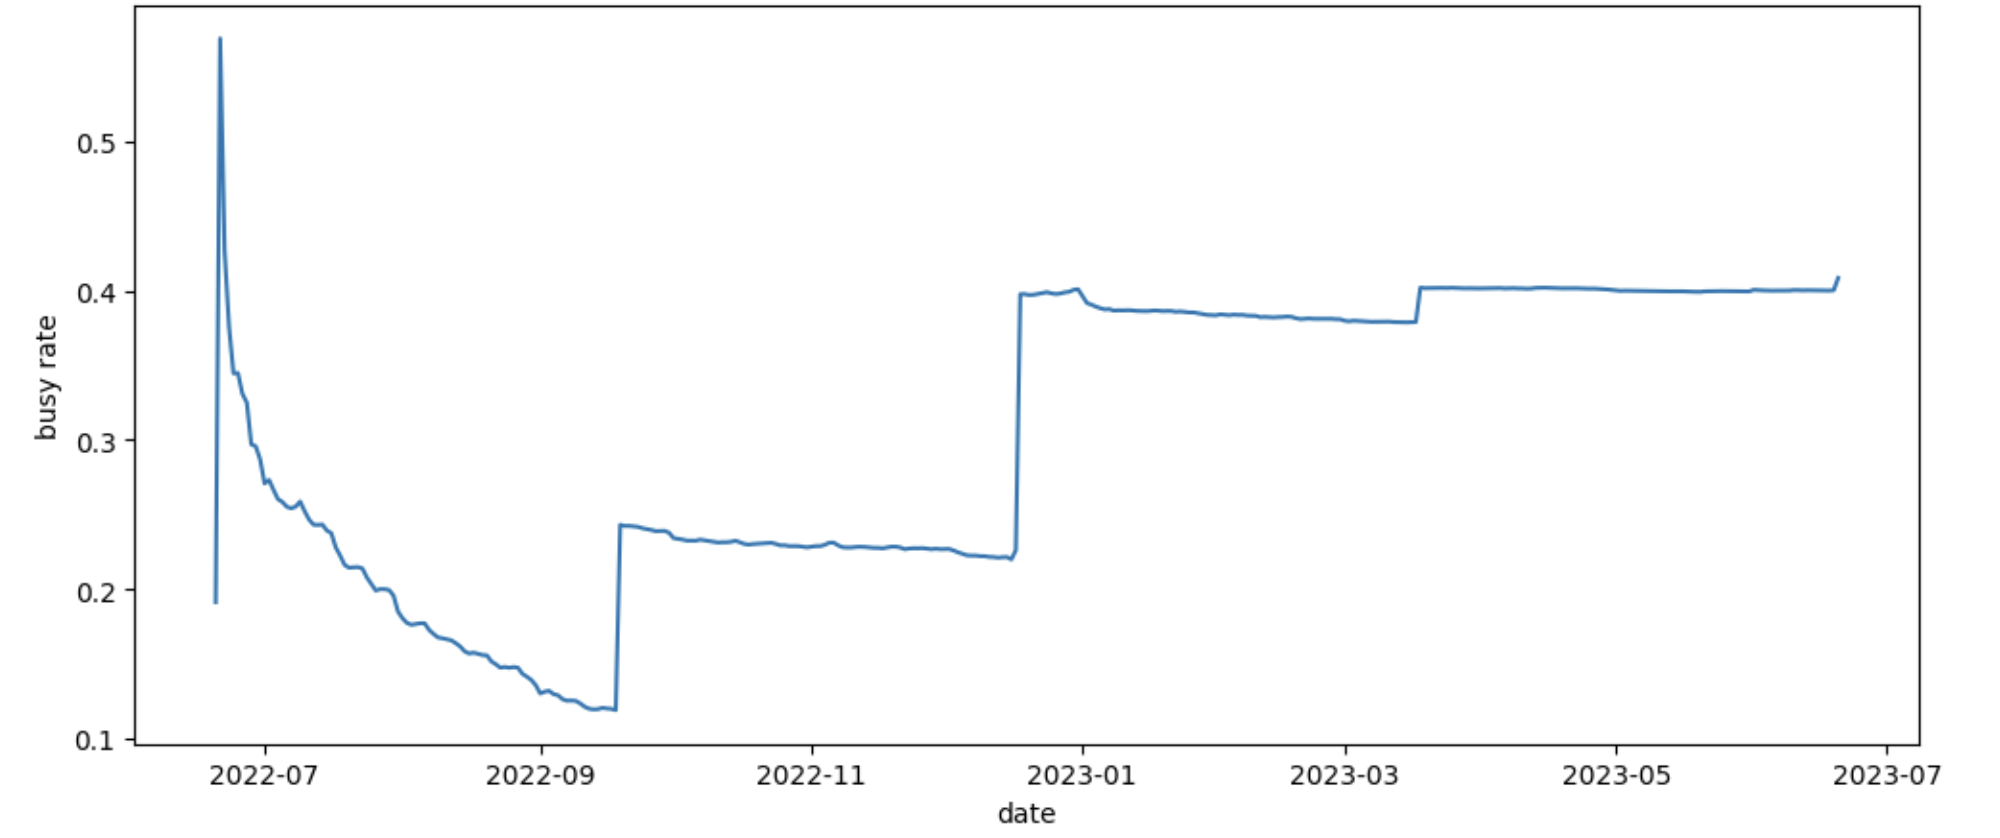
\includegraphics[width=.43\textheight]{busy_rate_year.png}
		\caption{Busy Rate within Year, $busy\  rate := \frac{\# (non-available\ rentals)}{\# (all\  rentals)}$}
		\label{fig:003}
	\end{figure}
	\newpage
	\noindent
	To illustrate this, there are \textbf{2 main things} in Figure \ref{fig:003}:
	\vspace{3pt}
	\\
	1. \textbf{Focus on the curve from '2022-07' to '2022-09'}, we will achieve some guideline for our customers (app users). That is, there are many rentals which are available if you reserve about one or two months before.
	\\
	2. It can be observed that, there are \textbf{abnormal step-shape curve} after '2022-09'. This is mainly because, the 'availabilty' is not only because some customers book this rental on that day, but also the hosts set the rental as 'available'. If the day is far away from today, hosts are more likely to set the rental as 'non-available'.
	\subsection{listings}
	Also, we firstly make some description to the 'listings' dataset.
	\vspace{3pt}
	\\
	1. There are 2 different datasets with respect to listing records, 'listings' and 'listings\_summary'. The difference is, 'listings\_summary' contains important parts of attributes. Therefore, we \textbf{use 'listing\_summary' for EDA} to achieve better sense of data and \textbf{use 'listings' to do data cleaning} and transform them into database.
	\\
	2. The 'listings' dataset is mainly about, the listing rental and its \textbf{all types of information} \textbf{(we will discuss in details below).} We can see all these information when we click one specific listing rental.
	\vspace{3pt}
	\\
	Then, we start to show the discovery results and some interesting observation:
	\subsubsection{Host-side information exploration}
	Here, we mainly focus on\textbf{ the distribution of \textit{counting number} of rentals in Airbnb that one host has}. The histogram diagram can be shown in Figure \ref{fig:004}:
	\begin{figure}[h]
		\centering
		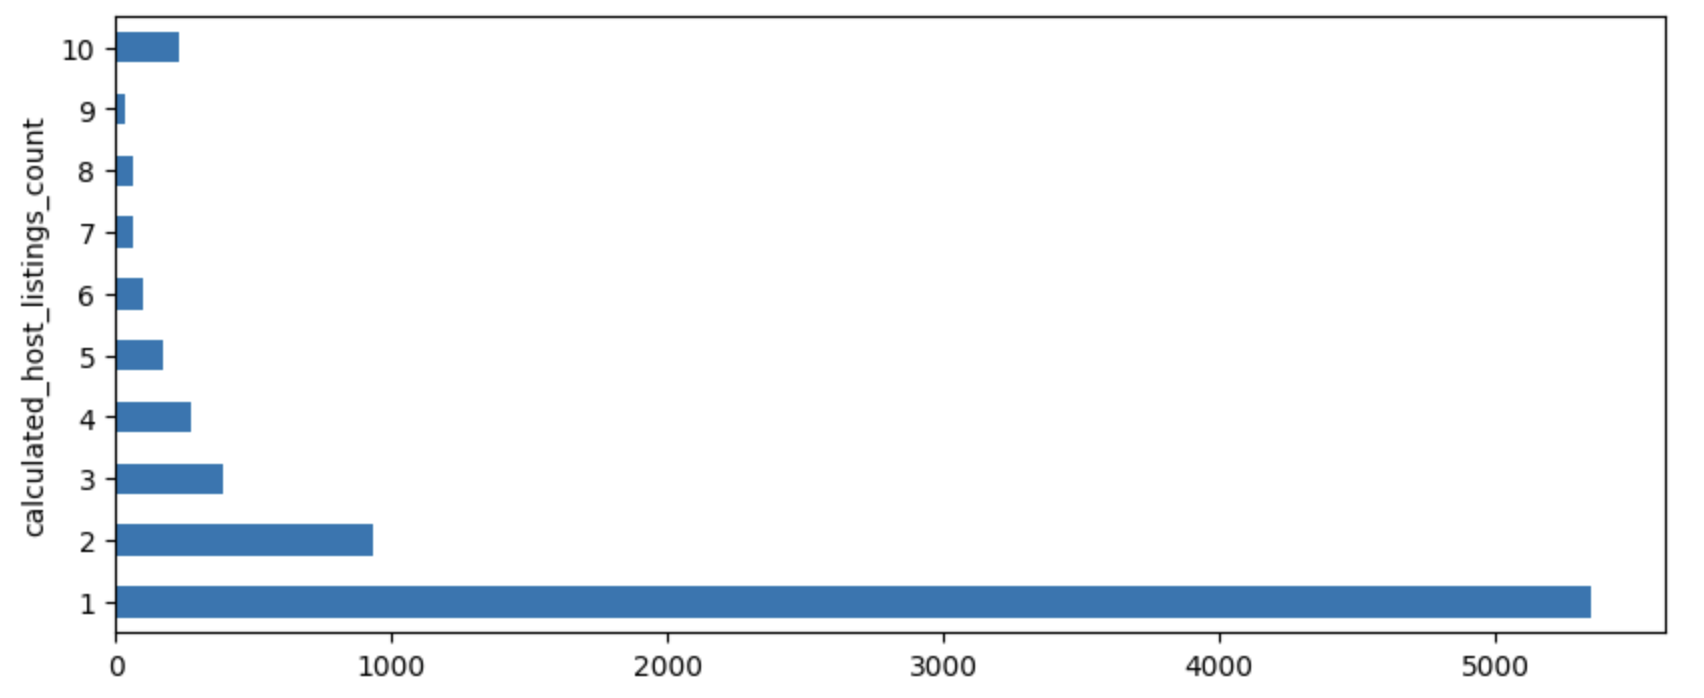
\includegraphics[width=.45\textheight]{host_side.png}
		\caption{Distribution of Rental Number One Host Has}
		\label{fig:004}
	\end{figure}
	\\
	It can be easily seen from Figure \ref{fig:004} that, the majority of hosts only have 1 rental in Airbnb. This piece of information may help \textbf{business side better understands those hosts and locate anomalies}.
	\subsubsection{Neighbourhood-side information exploration}
	Here, we focus on the \textbf{distribution of\textit{ couting number} and \textit{price} for rentals in different neighbourhoods}. The results can be shown as follows:
	\begin{figure}[h]
		\centering
		\subfigure[Boxplot of Price v.s. Neighbourhood]{
			\label{fig:subfig:a} %% label for first subfigure
			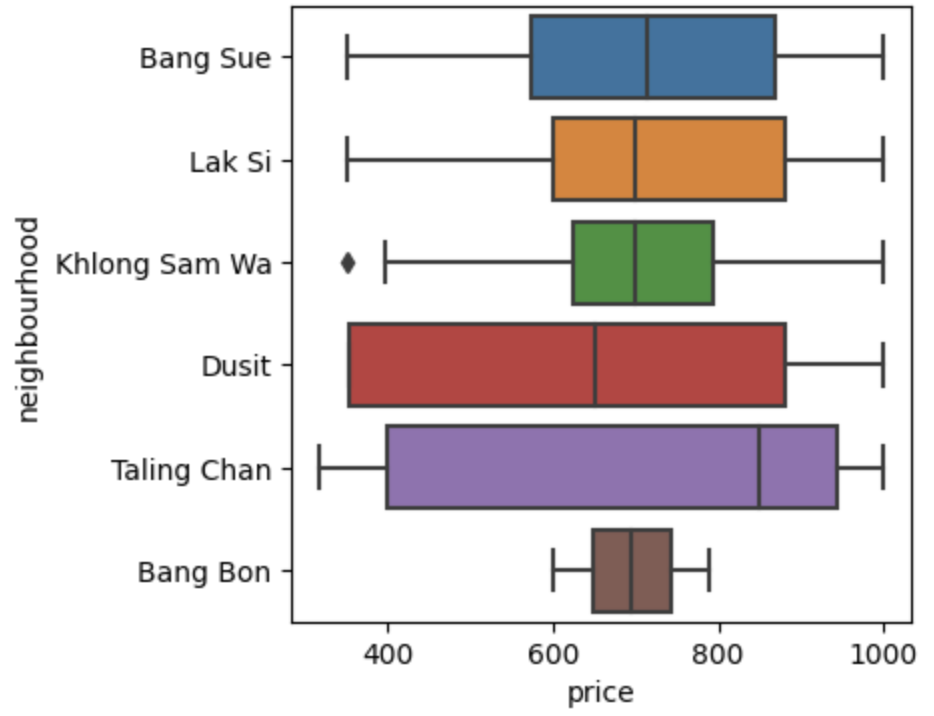
\includegraphics[width=2in]{neighb_1.png}}
		\subfigure[Line Chart of Price v.s. Neighbourhood]{
			\label{fig:subfig:b} %% label for second subfigure
			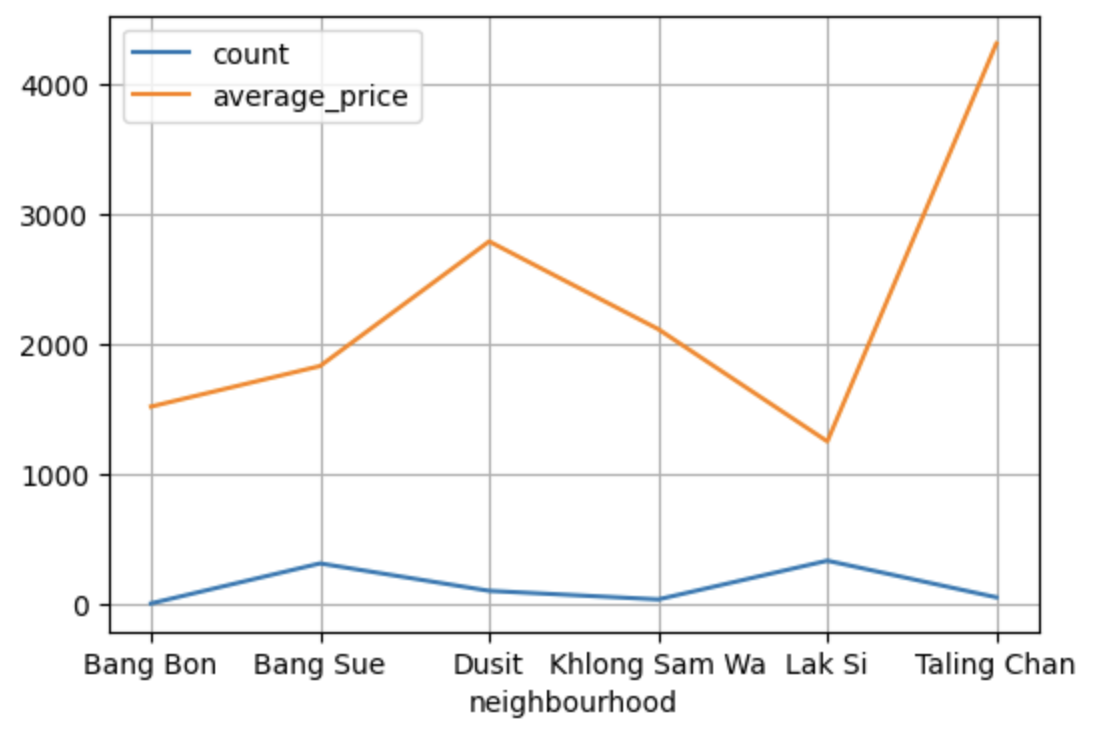
\includegraphics[width=2.3in]{neighb_2.png}}
		\caption{Visualization for Neighbourhood-side Information}
		\label{fig:005} %% label for entire figure
	\end{figure}
	\newpage
	\noindent
	1. In Figure \ref{fig:subfig:a}, it can be observed that, in different neighbourhoods, the variance of price is quite different. Take\textbf{ 'Tailing Chan' }as one example, the standard deviation of the price is quite big. This means, if you want to find one rental in that region, then \textbf{you should spend more time in comparing} because the variance of price is very big. On the other side, if you want to find rentals in \textbf{'Bang Bon'}, then you can spend less time since the price behaves quite similar. \textbf{As for the company}, these kinds of suggestions can be given to the app users to improve their app experience. 
	\\
	2. In Figure \ref{fig:subfig:b}, we mainly focus on \textbf{different price behaviours across regions}. You can see that,\textbf{ the number of rentals are quite imbalance across regions}. Buisness-side might need this information to optimize user experience.
	\subsubsection{Basic information exploration}
	Here, our interest is, the \textbf{relationship between \textit{number of bedrooms} and \textit{price}}. Something interesting has been discovered during the analysis. The whole exploration process will be included. Firstly, we visualize the relationship through boxplot in Figure \ref{fig:006}:
	\begin{figure}[h]
		\centering
		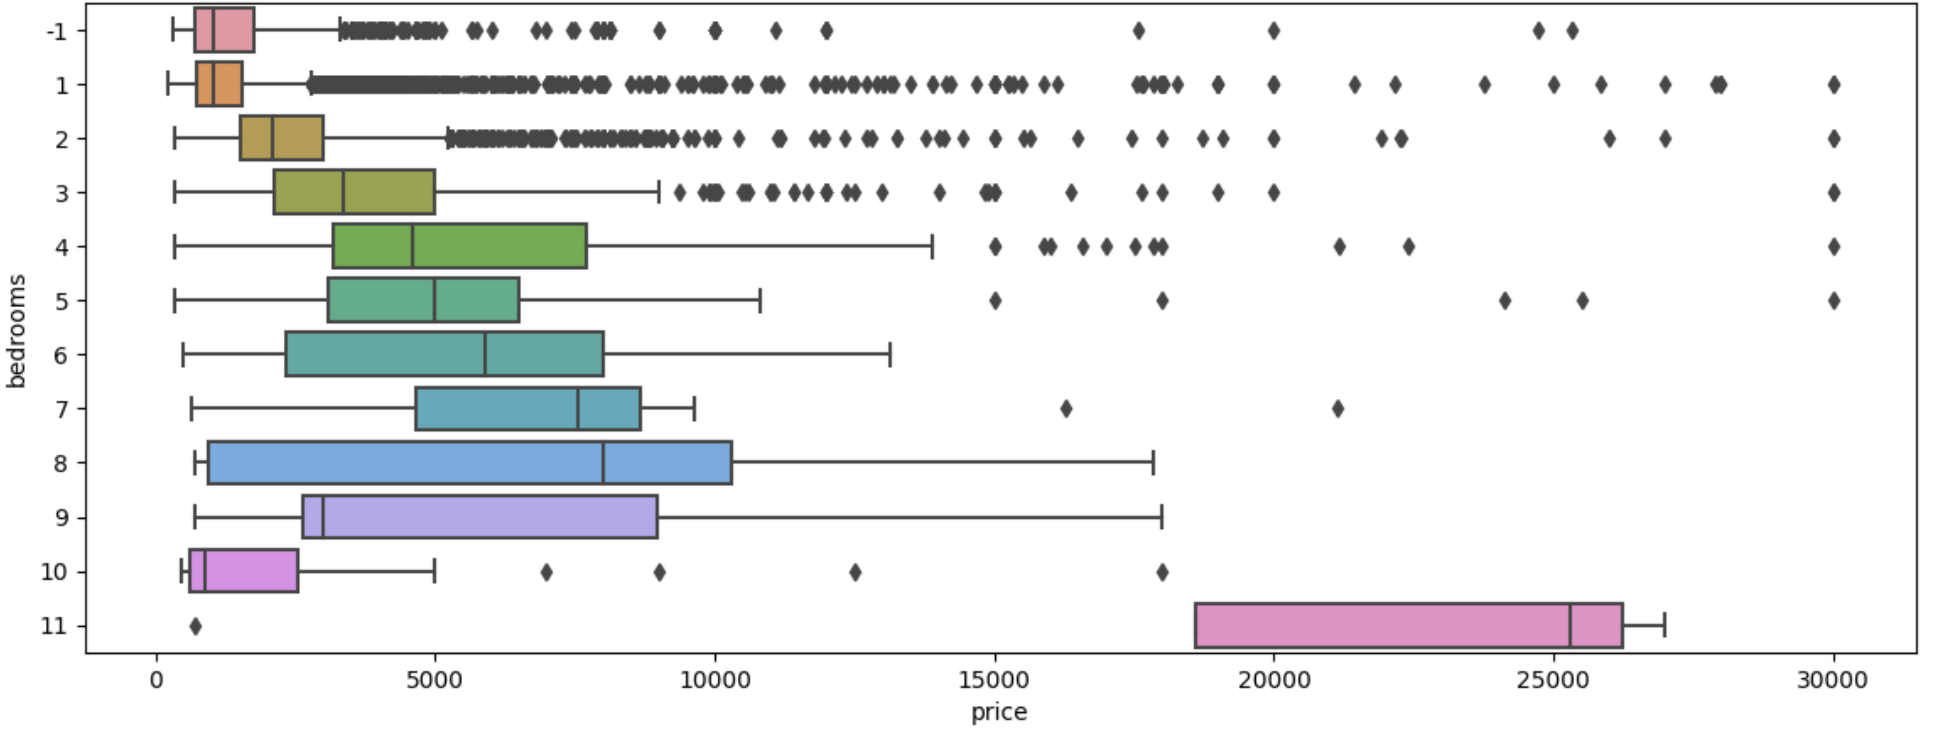
\includegraphics[width=.4\textheight]{price_bednum.png}
		\caption{Relationship between Price and Bedroom Number}
		\label{fig:006}
	\end{figure}
	\\
	To illustrate this, you can see that, except for \textbf{'bedroom = 9, 10'}, there \textbf{exists positive relationship} between \textbf{price} and \textbf{number of bedrooms}. However, a natural question is: \textbf{What happened for those rentals which have 9 or 10 bedrooms? } We \textbf{dive into the data to answer this}. In order to find an answer, we check those listings which have 10 bedrooms in details. The result is shown as follows:
	\begin{figure}[h]
		\centering
		\subfigure[10-Bedrooms Example]{
			\label{fig:subfig:c} %% label for first subfigure
			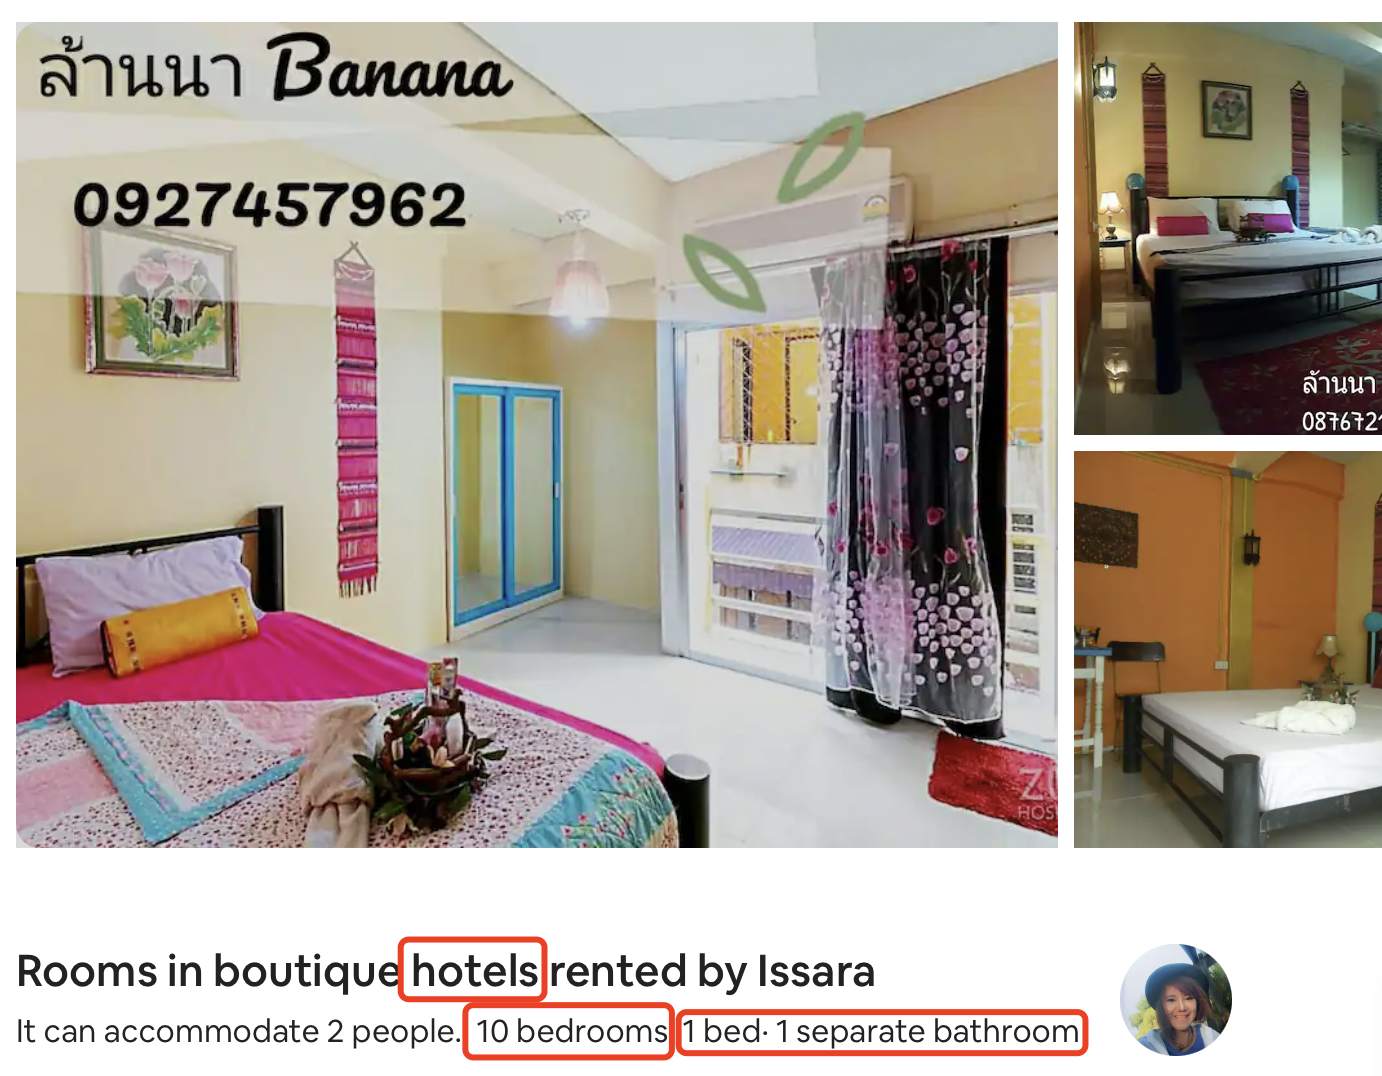
\includegraphics[width=2in]{further_check_1.png}}
		\subfigure[11-Bedrooms Example]{
			\label{fig:subfig:d} %% label for second subfigure
			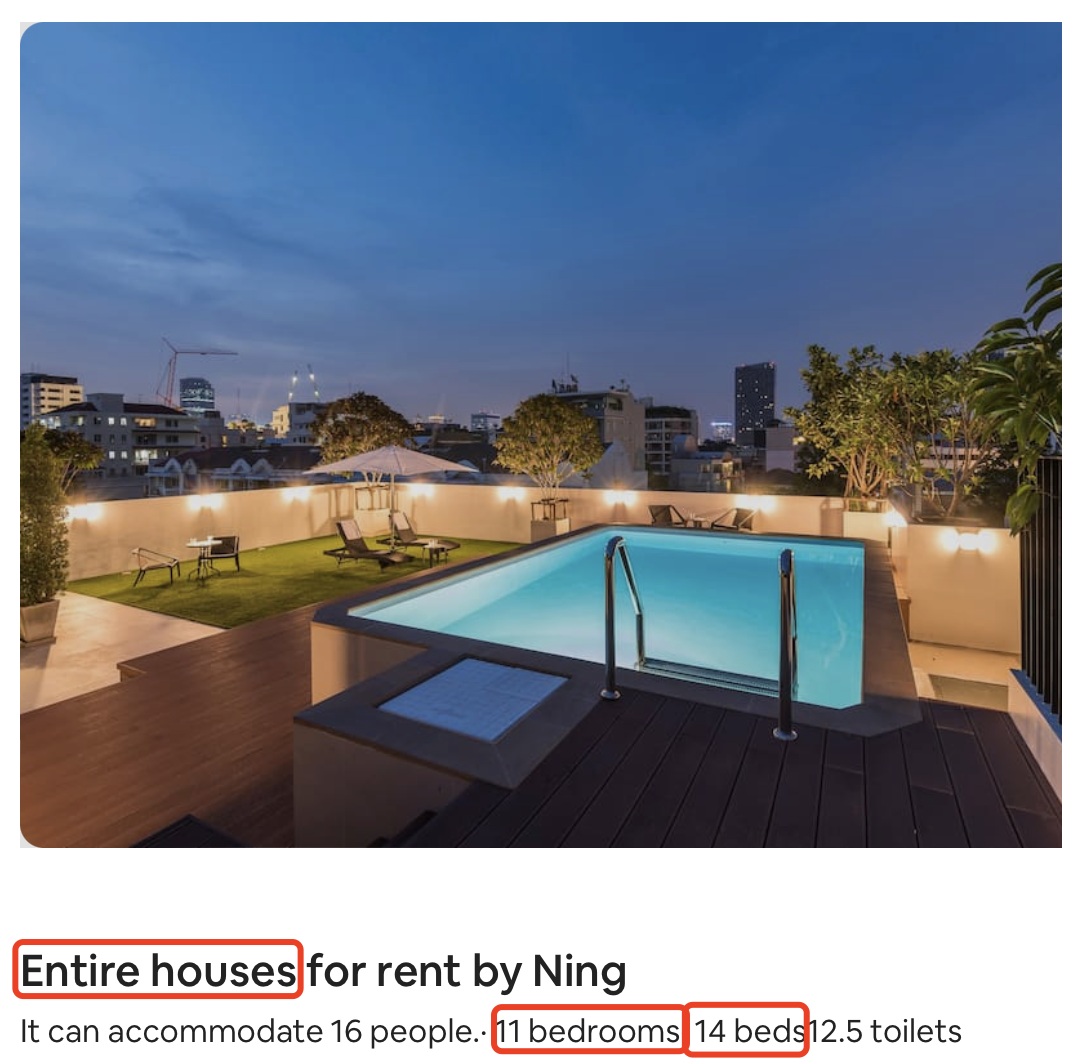
\includegraphics[width=1.8in]{further_check_2.png}}
		\caption{Exploration Result for 10-Bedrooms Case}
		\label{fig:007} %% label for entire figure
	\end{figure}
	\\
	In Figure \ref{fig:subfig:c}, you can see that, the type of this rental is hotel, and in the whole hotel, there are totally 10 rooms. \textbf{This is not what we want} with respect to the definiton of number of bedrooms. To compare, in Figure \ref{fig:subfig:d}, this rental has totally 11 bedrooms, which is a villa. This number is indeed what we want to tell customers.
	\vspace{3pt}
	\\
	Besides, after further checking, almost all the '10-Bedrooms' cases belong to this senario. Therefore, we can make conclusion that, most of the \textbf{'10-Bedrooms'} cases are due to the \textbf{data issues}. That is why their price is much lower than expected. After observing this, there are \textbf{2 insights from the exploration process}:
	\vspace{3pt}
	\\
	1. Those hosts should change 9 or 10 bedrooms to 0 bedroom if it is just a hotel;
	\\
	2. If we want to \textbf{make prediction} for price, then it is \textbf{better to use 'accomodates' attribute} in dataset.
	\subsection{reviews}
	Similarly, we firstly make some description with respect to the 'reviews' dataset.
	\vspace{3pt}
	\\
	1. There are 2 different datasets with respect to reivews records, 'reviews' and 'reviews\_summary'.\textbf{ The difference and our solution have been described in 'listings' case and we omit here}. 
	\\
	2. The dataset gives us information about, \textbf{all review records corresponding to each rental in given day}. This pieces of information will be displayed when we realize the 'review' function in the details of each rental. 
	\\
	3. The reviews information is recorded in multiple kinds of languages.
	\vspace{3pt}
	\\
	The detailed discovery results and some intuitive comments can be shown as follows:
	\subsubsection{Comment languages exploration}
	Here, we focus on\textbf{ the languages which are used in \textit{comments}}. This will help \textbf{business side} better understand our customers. The histogram diagram can be shown in Figure \ref{fig:008}:
	\begin{figure}[h]
		\centering
		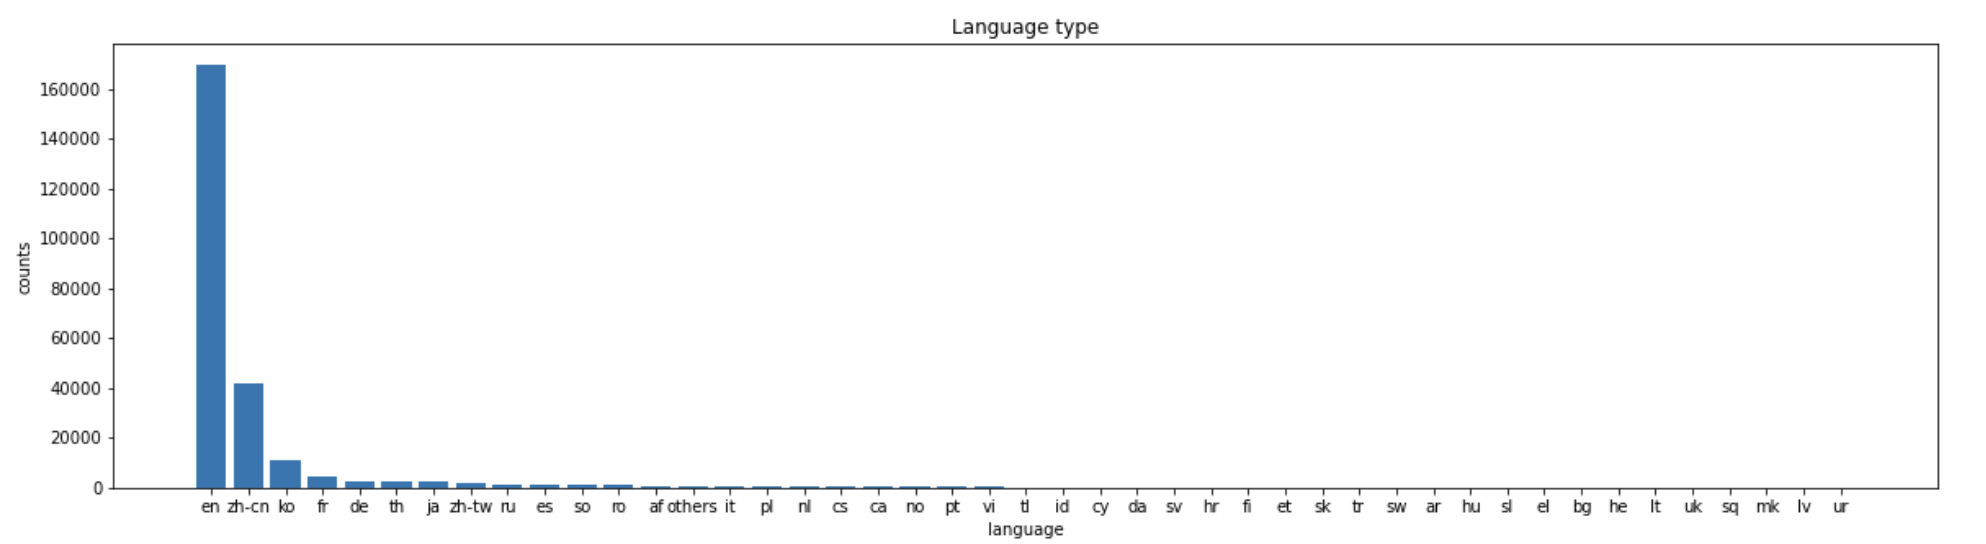
\includegraphics[width=.6\textheight]{language_type.png}
		\caption{Different Languages Used in Comment}
		\label{fig:008}
	\end{figure}
	\\
	It can be seen from Figure \ref{fig:008} that, majority of our customers use English and Chinese in their daily life. This can give us \textbf{some insights about the distribution of our customers}. 
	\vspace{3pt}
	\\
	Moreover, this also tells us that, \textbf{'comment'} attribute is not so clean. We may further ask tech-team to convert all languages into English and save them in database. This will bring great convenience for further NLP tasks if possible.
	\subsubsection{Brushing fraud exploration}
	Here,our interest is, \textbf{the fraud pattern hidden from \textit{number of review records} for rental and reviewer}. We will go through the whole process of how we find this. 
	\vspace{3pt}
	\\
	Firstly, we try to check the\textbf{ top 20 customers with most comments}. The visualization result is shown as follows:
	\begin{figure}[h]
		\centering
		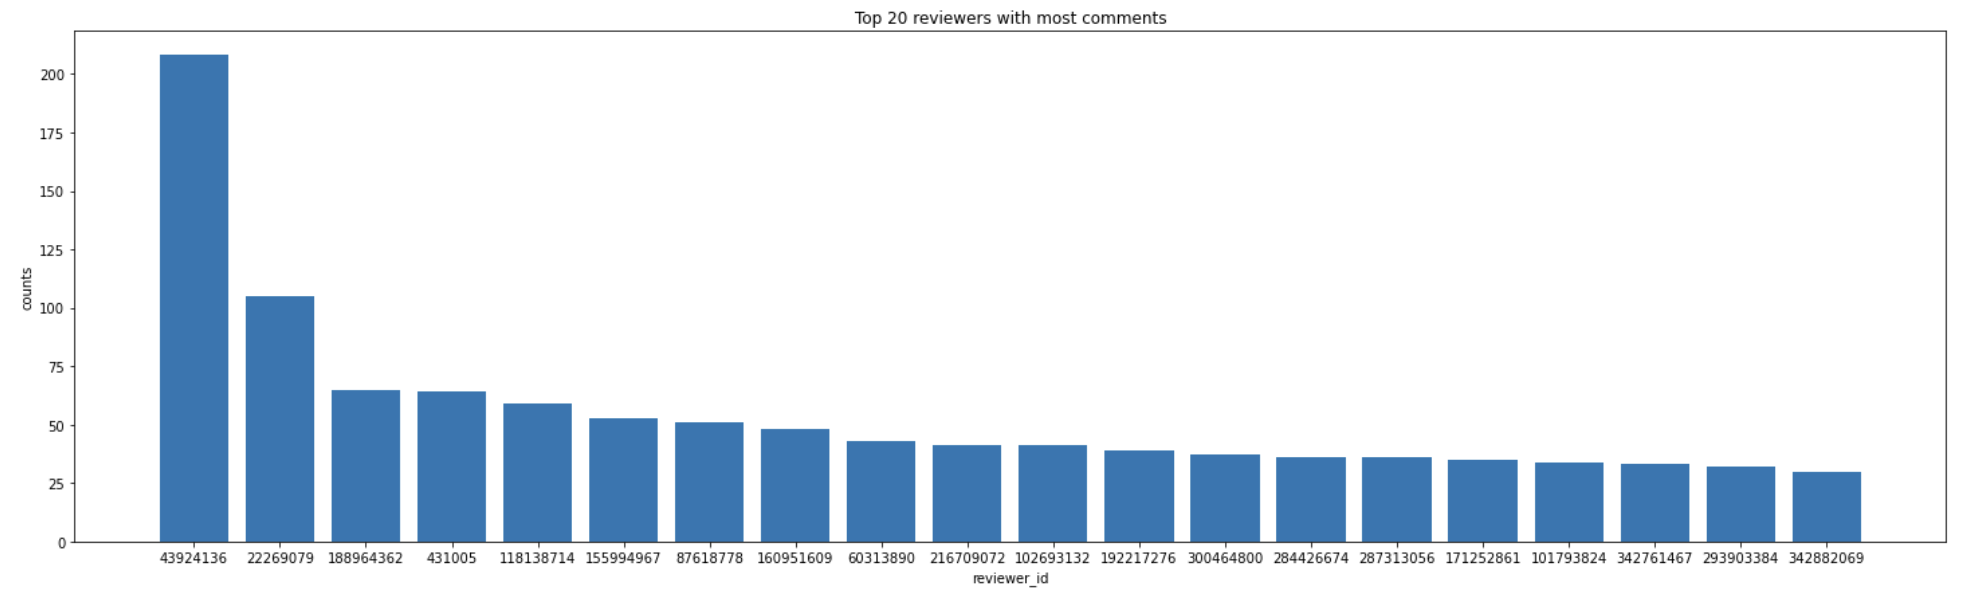
\includegraphics[width=.6\textheight]{top_20_reviewers.png}
		\caption{Top 20 Reviewers}
		\label{fig:009}
	\end{figure}
	\\
	In Figure \ref{fig:009}, the \textbf{number of comments} from\textbf{ top 1 reviewer} with most comment is extremely larger that from other reviewers. This is an abnormal observation since it is almost \textbf{impossible} for one normal customer to \textbf{book rentals so many times}.
	\vspace{3pt}
	\\
	To make it clear, we dive into more details about this 'abnormal' customer, saying that those review records from \textbf{'43924136 customer'}. The following Figure \ref{fig:010} tries to \textbf{compare }his review records with another customer who also has many review records (\textbf{'431005 customer'}):
	\begin{figure}[h]
		\centering
		\subfigure[Customer '43924136']{
			\label{fig:subfig:e} %% label for first subfigure
			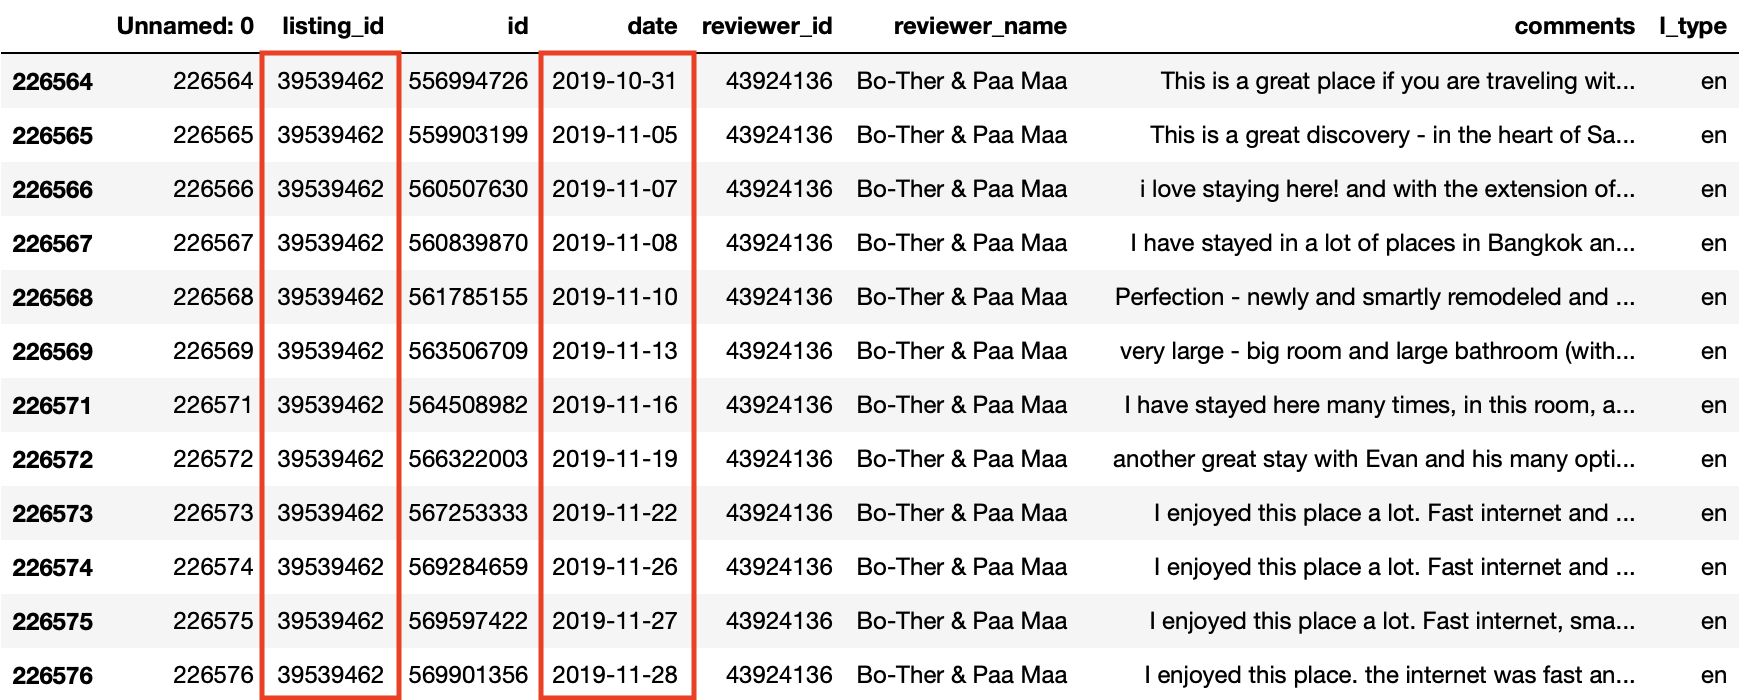
\includegraphics[width=3in]{cust1.png}}
		\subfigure[Customer '431005']{
			\label{fig:subfig:f} %% label for second subfigure
			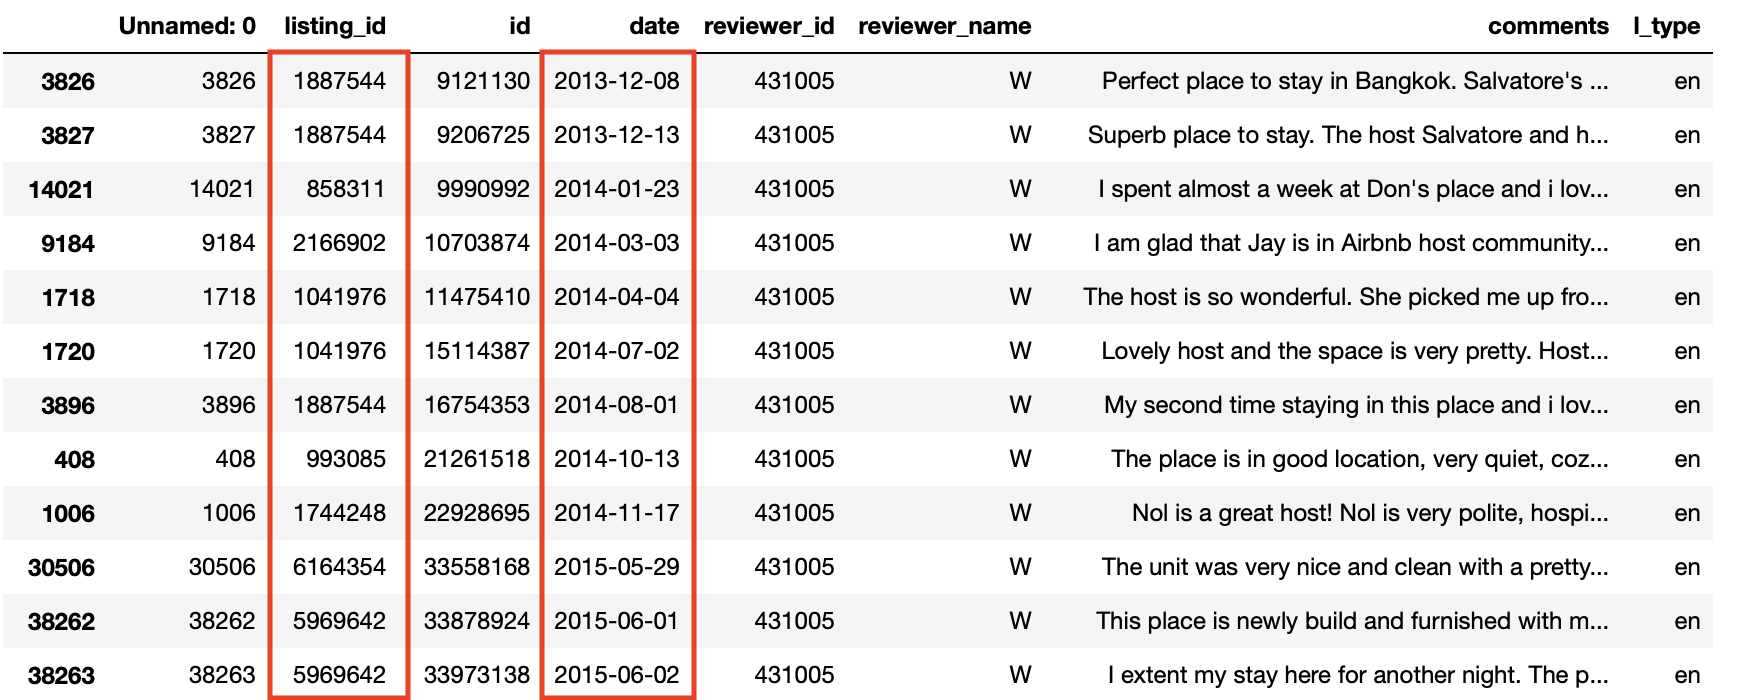
\includegraphics[width=3in]{cust2.png}}
		\caption{Reviews Comparison between 2 customers}
		\label{fig:010} %% label for entire figure
	\end{figure}
	\\
	To illustrate, in Figure \ref{fig:subfig:e}, it can be apparently observed that, the\textbf{ frequency of comments is much higher}, almost 2 or 3 times per week. Moreover, all the comments \textbf{contribute to the same rental}, which is very abnormal. In Figure \ref{fig:subfig:f}, the comment behavior is much more normal. That is, the \textbf{frequency of comments is much slower}, about six times per year. Besides, all the comments \textbf{contribute to different rentals}.
	\vspace{3pt}
	\\
	Therefore, we can conclude that, there may exist \textbf{Brushing Fraud} within review comments, which is similar to what \textbf{'43924136 customer' }does in the previous discussion. This piece of information can be sent to business side to consider further steps, including setting rules or building models to do detection.
	\subsection{relationship across 3 datasets}
	Lastly, we will briefly discuss the relationship among 3 datasets, especially the referential constraints. 
	\vspace{3pt}
	\\
	1. In 'calendar' dataset, the 'listings\_id' attribute references to the 'id' attribute in 'listings';
	\\
	2. In 'reviews' dataset, the 'listings\_id' attribute references to the 'id' attribute in 'listings'. 
	\vspace{5pt}
	\\
	\textbf{Remark:} Besides above 4 parts, we also \textbf{do other exploration }with respect to the 3 datasets. Moreover, \textbf{analysis on the data types} have also been done during the exploration process. For simplicity, the details of these results will be attached in the \textbf{Appendix}. Here, we only display those meaningful exploration.
	
	\section{Data Cleaning}
	In this section, we will clean three datasets, i.e., 'calendar', 'listings', and 'reviews' step by step. We will mainly focus on dataset 'listings' since it is most sophisticated and troublesome.  
	
	\subsection{Null Value}
	First we count the null values grouped by columns and show the results as follows.
	\\
	\begin{table}[h]
		\centering
		\begin{tabular}{cc}
			\toprule
			Column Name                    & Null Value Counts \\
			\midrule
			bathrooms                      & 17074             \\
			license                        & 17074             \\
			calendar\_updated              & 17074             \\
			neighbourhood\_group\_cleansed & 17074    \\  \bottomrule      
		\end{tabular}
		\caption{Null value counts in dataset listings where all values are missing.}
	\end{table}
	
	
	\noindent We find that all data in column 'bathrooms', 'license', 'calendar\_updated' and 'neighbourhood\_group\_cleansed' are missing. Therefore, we drop all these four columns out of the database.
	
	\noindent While for the result columns, only partial data is missing. We keep all these data for sake of data integrity.
	
	\begin{table}[h]
		\centering
		\begin{tabular}{cc}
			\toprule
			Column Name                                           & Null Value Counts \\
			\midrule
			neighborhood, neighborhood\_overview & 7615              \\
			review\_scores\_value                                    & 7296              \\
			review\_scores\_cleanliness, review\_scores\_accuracy    & 7288              \\
			host\_neighbourhood                                      & 7262              \\
			reviews\_per\_month, first\_review                       & 7062              \\
			review\_scores\_rating, last\_review                     & 7062              \\
			host\_acceptance\_rate                                   & 6779              \\
			host\_response\_time, host\_response\_rate               & 5629              \\
			bedrooms                                                 & 1703              \\
			description                                              & 905               \\
			host\_location                                        & 44                \\
			name                                                  & 9                 \\
			host\_listings\_count, host\_picture\_url             & 2                 \\
			host\_thumbnail\_url, host\_is\_superhost             & 2                 \\
			host\_total\_listings\_count, host\_has\_profile\_pic & 2                 \\
			host\_identity\_verified, host\_since, host\_name     & 2                 \\
			maximum\_minimum\_nights, maximum\_nights\_avg\_ntm   & 1                 \\
			\bottomrule
		\end{tabular}
		\caption{Null value counts in dataset listings where partial data is missing (part).}
	\end{table}
	\subsection{Find/delete special characters}
	Since the data is crawled down from the website, it inevitably contains some dirty information. We detailed check every column, and conduct series of operations on the corresponding column:
	\vspace{3pt}
	\\
	1. 'host\_verifications'. We drop quotation marks and brackets and only keep the items like 'email', 'phone' and 'work\_email'.
	\\
	2. 'amenities'. We decode every string with 'utf-8' and find something error caused by escape sequence like \textbackslash n and \textbackslash t. Besides, we also find some noise information like xx\textbackslash \textbackslash, where xx are two consecutive numbers. We drop these characters by regular expression. 
	\\
	3. 'description', 'neighborhood\_overview', 'neighbourhood', and 'host\_about'. For these four columns, we detect blank unicode like \textbackslash xa0 and \textbackslash u3000 and some tags like \textless \textbackslash br \textgreater or similar formats from HTML files. We also drop all these characters by regular expression. 
	\subsection{Change format from string to boolean, float, and int}
	
	We convert the following columns to corresponding data types. We show the results in table \ref{table:data_type}.
	
	\begin{table}[h]
		\centering 
		\begin{tabular}{cc}
			\toprule
			Column                                                         & Data type \\
			\midrule
			host\_is\_superhost, host\_has\_profile\_pic                   & Boolean   \\
			host\_identity\_verified, has\_availability, instant\_bookable & Boolean   \\
			price, host\_response\_rate, host\_acceptance\_rate            & Float     \\
			latitude, longitude,review\_scores\_rating                     & Float     \\
			review\_scores\_cleanliness, review\_scores\_checkin           & Float     \\
			review\_scores\_communication, review\_scores\_location        & Float     \\
			review\_scores\_value, reviews\_per\_month                     & Float     \\
			minimum\_nights\_avg\_ntm, maximum\_nights\_avg\_ntm           & Float \\
			the rest & Int \\
			\bottomrule
		\end{tabular}
		\caption{Columns and corresponding data types.}\label{table:data_type}
	\end{table}
	
	\subsection{Set ';' as separator}
	Usually, people set comma as separator in csv file. However, in our project we have many descriptive columns containing text information and comma. Therefore, when loading the data to database, the system will mistake the comma inside the text for the separator. 
	\noindent In our project, we solve this problem by using ';' as the only separator. For the same reason, an very important step is to convert other ';' in text to ',' such that ';' in text will not influence data loading process.
	
	\subsection{Summary for data cleaning}
	We also do the similar operations for the other two datasets. Such process is much simpler comparing to dealing with dataset 'listing'. Despite the loss and change of some characters and punctuation, we try our best to uniform the format and keep the original data including, but not limited to, more than 40 languages, and emoji. 
	
	
	\section{Data Generation}
	In this section, we will generate some artificial transaction data based on dataset reviewer. We do this in the following way.
	\vspace{3pt}
	\\
	1. First, We tend to generate 20\% of the total comments as source of transaction data. Each comment is associated with a host, a listing, and time stamp. We fix the random state and sample from the original data. 
	\\
	2. Second, we generate end date for each transaction. For simplicity, we set the reviewing date as the start date for each transaction. The end date is determined by the stay time that each client spent. Based on actual needs, we generate the stay time using a specified distribution in which the probability for one-day stay is 30\% and two-week stay is 1\%.
	\\
	3. Last, we generate booking price for each transaction.That is, we check the corresponding average booking price in the following year and set it as the cost per day index and thus generate the total cost. 
	
	\section{Requirement Analysis}
	As we mentioned, we will conduct the analysis from 2 different scenarios, \textbf{naive user level} and \textbf{host level}.
	\subsection{Naive user level}
	From the real-life perspective, naive users, i.e., those Airbnb app users, they will focus on things like, searching for the rental that satisfies some condition and viewing the information about one speicific rental etc..
	\vspace{3pt}
	\\
	To conclude, there are \textbf{4 main requirements} for naive users:
	\vspace{3pt}
	\\
	1. \textbf{Searching function}. 
	\\
	That is, given some condition like price and room type, \textbf{return those rental satisfying these conditions}. Moreover, the return can be sorted by some attributes of the rental like review scores. 
	\\
	Moreover, someone might be interested in some super-hosts for their aesthetic. Then, it is necessary for us to \textbf{return the list of most popular} super-hosts if users want.
	\vspace{3pt}
	\\
	2. \textbf{Viewing function for rental}. 
	\\
	In this part, users want to see \textbf{all kinds of information about one specific rental}, including its neighbourhood, price, amenities and so on.
	\\
	For example, one may want to \textbf{check whether one rental is available }during some time period in order to make further decision about their trip. Also, to compare between 2 rentals, users can view the review records to make their decision. We think the latter situation is very important in every user's experience life.
	\vspace{3pt}
	\\
	3. \textbf{Viewing function for host}.
	\\
	Here, users can \textbf{check all the details of one specific host}, including his/her basic information, all review records and rental information to make better choices. This will give users a easier way to find more rentals.
	\vspace{3pt}
	\\
	4. \textbf{Viewing function for transaction.}
	\\
	Customers may want to check their \textbf{previous transaction records}, which should be one basic function for users' experience. 
	\subsection{Host level}
	As for hosts, for each of their rental, they need to assign one price. Thus, they may want some guideline from our side. Also, they might be interested in the function which can clearly display the orders of their rentals. We can show them the details of these information to support them.
	\vspace{3pt}
	\\
	To conclude, the \textbf{2 main requirements} for hosts are:
	\vspace{3pt}
	\\
	1. \textbf{Pricing-suggest function}.
	\\
	In this part, when hosts fill in their basic information about rental, they want some suggestions from us about the pricing. We can return prices from other hosts who have rental with similar basic information. Moreover, we can further \textbf{build Machine Learning model about price-prediction} to give better suggestions for their pricing decision.
	\vspace{3pt}
	\\
	2. \textbf{Dashboard function}.
	\\
	Here, hosts might be interested in, \textbf{a dashboard about his privous/future rental transaction records}. 
	\\
	Take one simple example, many hosts will want to know that, in the previous 3 months, all the \textbf{reservation results} for each of his rental. By achieving this, it can be of some help for hosts to arrange their time.
	\section{Relational Database Storage}
	After finishing the requirement analysis, we start to build up our relational database model. Here, \textbf{we use \textit{Mysql DBMS} to store our data}. The whole prcoess can be decomposed into, ER Diagram Deisgn, Schema Diagram Translation and Schema Refinement.
	\subsection{ER Diagram Deisgn}
	Before giving the ER Diagram, we first conduct analysis about Entity and Relationship for these 3 datasets:
	\vspace{3pt}
	\\
	\textbf{Entity:}
	\\
	hosts, reviewers, calender slots, listing rooms, transaction, comment;
	\vspace{3pt}
	\\
	\textbf{Relationship: }
	\\
	1. Binary: (host) holds (listing room), (listing room) has (calendar slot);
	\\
	2. 3-ary: CRL(comment, reviewer, listing room);
	\\
	3. 4-ary: TRHL(trasaction, reviewer, host, listing room);
	\vspace{3pt}
	\\
	Based on the above analysis, the ER Diagram can be shown in Figure \ref{fig:011}:
	\begin{figure}[h]
		\centering
		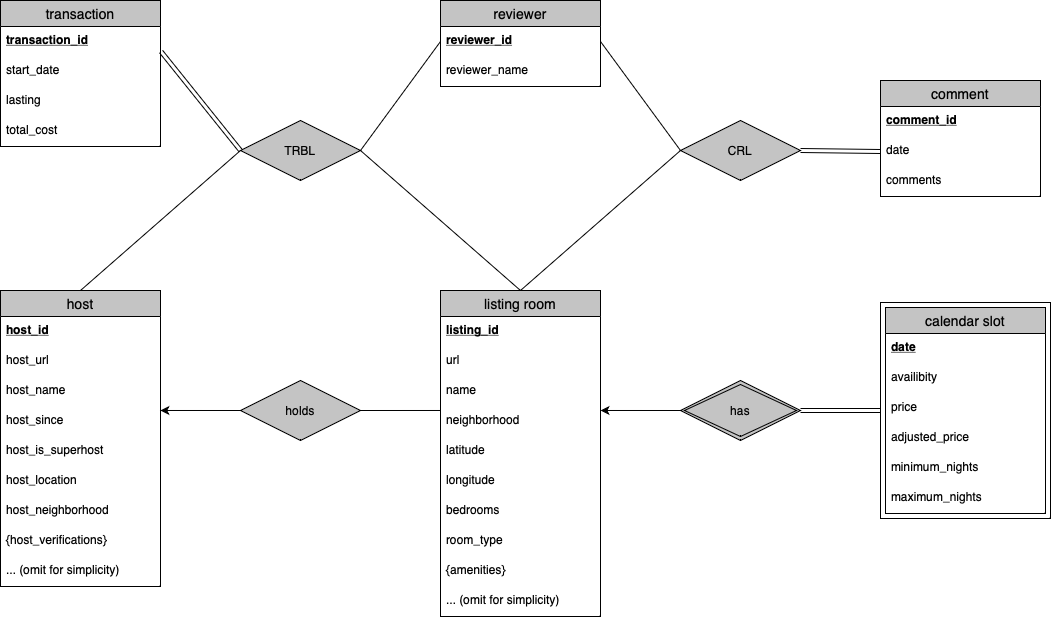
\includegraphics[width=.5\textheight]{er.png}
		\caption{Entity-Relationship Diagram}
		\label{fig:011}
	\end{figure}
	\vspace{3pt}
	\\
	There are \textbf{several explanations} with respect to Figure \ref{fig:011}, which can be listed as follows:
	\vspace{3pt}
	\\
	1. In \textbf{'listing room' entity set}, the \textbf{'amenities'} attribute is \textbf{multi-valued type}. Therefore, to convert this to schema diagram, we should create a new relation (table) to store (listing\_id, amenity) pairs (same as \textbf{'host\_verfications' in 'host' entity set});
	\vspace{3pt}
	\\
	2. In 4-ary 'TRHL' relationship, we can view this as one \textbf{many-to-one relationship} and \textbf{'transaction' entity set is in the many side}. That is to say, \textbf{each transaction entity corresponds to exactly one (reviewer\_id, host\_id, listing\_id) pair} (coming from the fact that 'transaction' entity set is totally participated).
	\\
	Therefore, when we convert this into schema diagram, we just need to \textbf{store the primary keys of 'reviewer', 'host' and 'listing room' in the 'transaction' side} instead of creating new tables.
	\vspace{3pt}
	\\
	3. Similarly, in 3-ary 'CRL' relationship, we can also view it as \textbf{many-to-one relationship} and \textbf{'comment' entity set is in the many side}. \textbf{Each 'comment' entity corresponds to exactly one (review\_id, listing\_id) pair}.
	\\
	Therefore, when converting to schema diagram, we only need to \textbf{store the primary keys of 'reviewer' and 'listing room' in the 'comment' side}
	\subsection{Schema Diagram Translation}
	Then, follow the above explanation, we can start to convert the ER Diagram into Schema Diagram. The converting result is shown in Figure \ref{fig:012}:
	\begin{figure}[h]
		\centering
		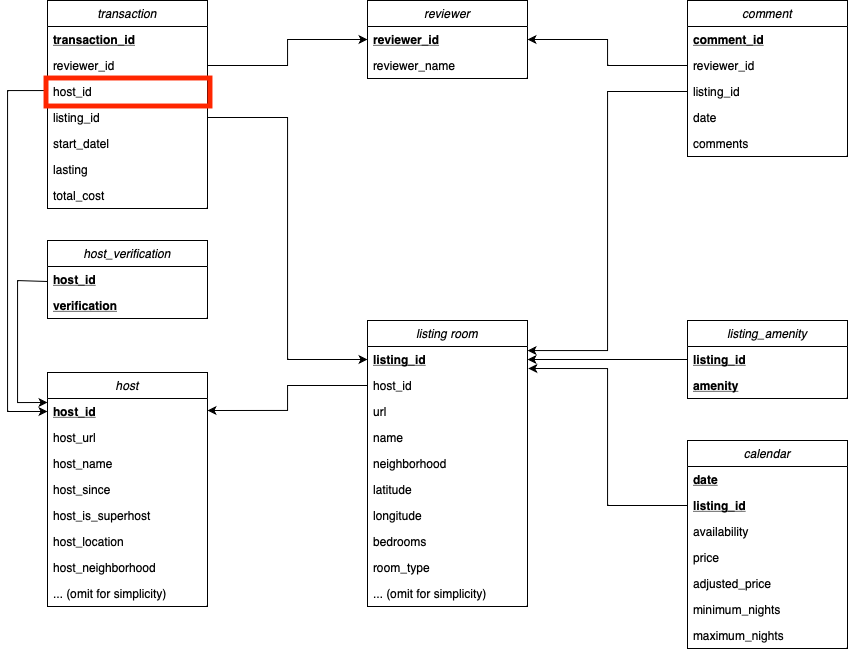
\includegraphics[width=.5\textheight]{sd.png}
		\caption{Schema Diagram}
		\label{fig:012}
	\end{figure}
	\vspace{3pt}
	\\
	There are some illustration with respect to the red frame in Figure \ref{fig:012}:
	\vspace{3pt}
	\\
	1. There are \textbf{some non-trivial Functional Dependencies} within \textbf{'transaction' }relation. That is, \textbf{'listing\_id' will determine 'host\_id'}, i.e., 
	$$
	'listing\_id' \implies 'host\_id'
	$$
	This is what we should consider when we make Schema Refinement.
	\subsection{Schema Refinement}
	In Figure \ref{fig:012}, we can be sure that, in 'host', 'reviewer', 'listing room', 'comment', 'listing\_amenity' and 'calendar' relation, there are no non-trivial FDs. The \textbf{only non-trivial FD for the whole database} is in \textbf{'transaction'} relation, which is:
	$$
	'listing\_id' \implies 'host\_id'
	$$
	\vspace{3pt}
	\\
	In order to achieve BCNF, we should decompose 'transaction' relation based on this FD. Moreover, observe that, in \textbf{'listing room'} relation, \textbf{this FD has already been included}. Therefore, we can \textbf{simply drop the 'host\_id' attribute} in 'transaction' relation to achieve BCNF.
	\vspace{3pt}
	\\
	The \textbf{Refined Schema Diagram} can be shown in Figure \ref{fig:013}:
	\begin{figure}[h]
		\centering
		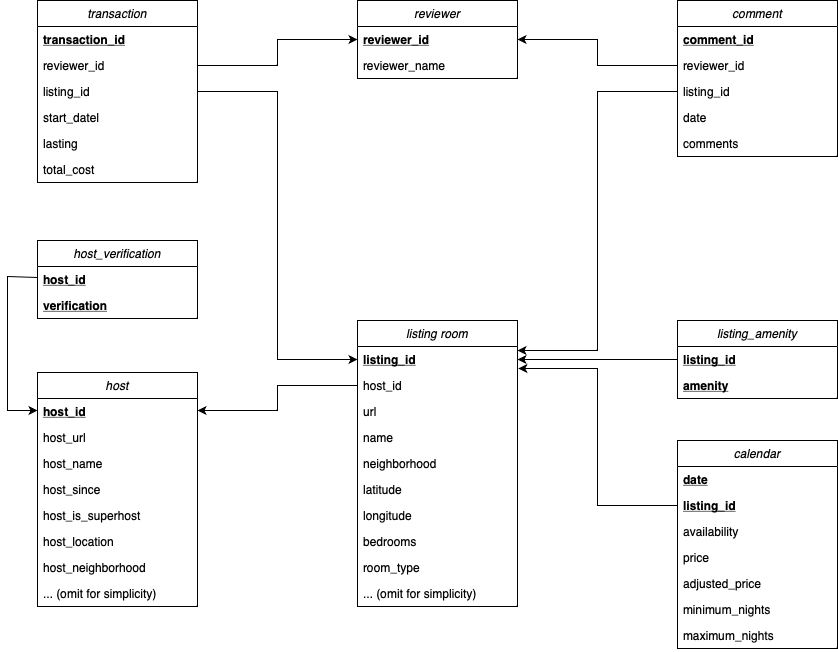
\includegraphics[width=.54\textheight]{sd_refine.png}
		\caption{Refined Schema Diagram (BCNF)}
		\label{fig:013}
	\end{figure}
	\\
	Based on all above analysis, \textbf{this database is in BCNF}! Then, we split the \textbf{cleaned data (4 .csv files)} into the form of Figure \ref{fig:013} and store them in \textbf{\textit{Mysql DBMS}}, which can be shown in Figure \ref{fig:014}:
	\begin{figure}[h]
		\centering
		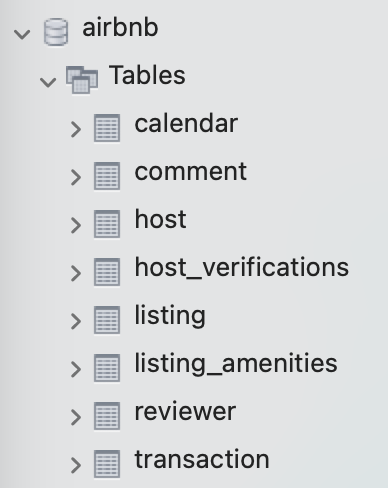
\includegraphics[width=.2\textheight]{mysql_db.png}
		\caption{Mysql Database}
		\label{fig:014}
	\end{figure}
	\\
	\section{Non-relational Database Storage}
	Firstly, we choose \textbf{\textit{MangoDB}} to implement the \textbf{Non-relational Database} since this is what we have learnt in lecture. Again, we start from ER Diagram and then transform it into MongoDB Schema. Based on the form defined in schema, we store the data into \textbf{\textit{MongoDB}}.
	\subsection{ER Diagram Recap}
	Firstly, let's recap the ER Diagram so that we can further build \textbf{well-organized }schema \textbf{acoording to the advantages} of \textbf{\textit{MongoDB}}. The diagram is shown as follows:
	\begin{figure}[h]
		\centering
		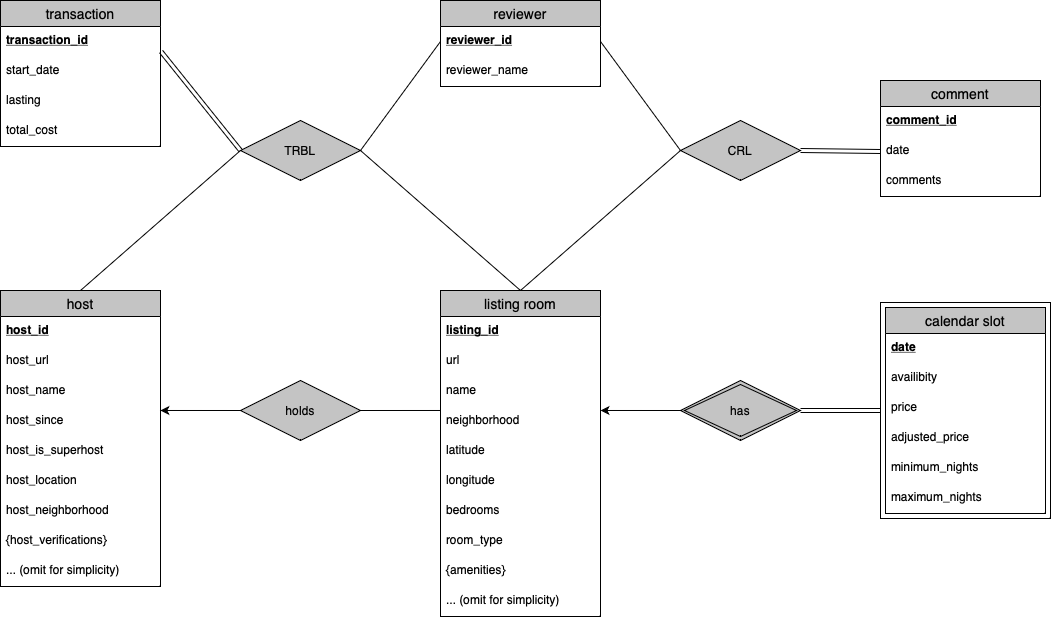
\includegraphics[width=.45\textheight]{er.png}
		\caption{Entity-Relationship Diagram}
		\label{fig:018}
	\end{figure}
	\\
	Actually, what we should do is to make a choice between\textbf{ 'embedding' and 'reference'} based on the property of each relationship. To conclude, there are 3 kinds of relationships in ER Diagram (Figure \ref{fig:018}):
	\vspace{3pt}
	\\
	1. 'TRBL' and 'CRL': n-ary "one-to-many" relationship with $n \ge 3$;
	\\
	2. 'holds' and 'has': 2-ary one-to-many relationship;
	\\
	3. 'host\_verfications' and 'amenities': multi-valued attributes which can be modelled as one-to-many relationship;
	\subsection{Schema Analysis}
	In the following discussion, we will give different recipes to each kind of relationship:
	\vspace{3pt}
	\\
	1. As for these n-ary relationships, it should be noticed that, each 'transaction\_id' ('comment\_id') will only correspond to unique foreign key pairs, i.e., ('host\_id',\ 'listing\_id',\ 'reviewer\_id'). In this fashion, it can be viewed as, 'transaction\_id' is on the 'many' side.
	\\
	Moreover, if we want to use \textbf{'embedding'} to model these 2 relationships, then \textbf{the nested term will be extremely long}. This suggests us that, \textbf{we should model these 2 relationships with respect to 'reference'}.
	\vspace{3pt}
	\\
	2. As for these 2-ary relationships, due to similar reason, we \textbf{recommend that these should be modelled as 'reference'}. Briefly speaking, \textbf{'one' side has too many attributes}, which \textbf{makes the 'embedding' formulation very 'heavy'}.
	\vspace{3pt}
	\\
	3. As for these 2 multi-valued attributes, \textbf{it should be modelled as 'embedding' because the 'one' side is very 'light'}. It can be easily nested into the json element.
	\subsection{Conclusion}
	According to previous discussion, now we can eventually determine the \textbf{\textit{MongoDB} Schema} as:
	\vspace{3pt}
	\\
	1. \textbf{'TRBL' and 'CRL', 'holds' and 'has': 'reference';}
	\\
	2. \textbf{'host\_verfications' and 'amenities': 'embedding'.}
	\newpage
	\noindent
	Moreover, then we split the \textbf{cleaned data (4 .csv files) into 6 collections (no host\_verfications and listing\_amenity)} and store them in \textbf{\textit{MongoDB DBMS}}, which can be shown in Figure \ref{fig:019}:
	\begin{figure}[h]
		\centering
		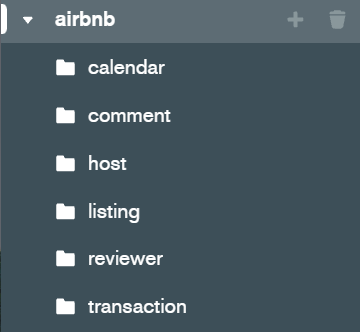
\includegraphics[width=.2\textheight]{mangodb_demo.png}
		\caption{MongoDB Database}
		\label{fig:019}
	\end{figure}
	\section{Query Answer}
	Before showing the results of queries, we say that, in order to achieve \textbf{better performance of query} (with respect to \textbf{efficiency}), \textbf{we set index for those important attributes}. That is, those attributes which are more likely to use for query.
	\vspace{3pt}
	\\
	Therefore, based on the Requirement Analysis as we talked about before, we display all natural language queries and their corresponding database queries as follows (\textbf{for simplicity, in all queries, we return 5 records}):
	\subsection{Relational Database}
	1. \textbf{Natural Language Query}: return 5 listings that are suitable for 3 people.
	\vspace{3pt}
	\\
	2. \textbf{Natural Language Query}: return 5 listings whose prices are between 500 and 700, combining with room type is private room.
	\vspace{3pt}
	\\
	3. \textbf{Natural Language Query}: return 5 hosts who belong to super hosts and their all listing rooms.
	\vspace{3pt}
	\\
	4. \textbf{Natural Language Query}: return 5 reservation records for the listing room whose id = '39539462' and date between '2022-07-31' and '2022-08-07'.
	\vspace{3pt}
	\\
	5. \textbf{Natural Language Query}: return 5 review records for the listing room whose id = '39539462'.
	\vspace{3pt}
	\\
	6. \textbf{Natural Language Query}: return 5 review records for the user  whose name = 'Nathan'.
	\vspace{3pt}
	\\
	7. \textbf{Natural Language Query}: return the basic information for the host whose name = 'Nathan'.
	\vspace{3pt}
	\\
	8. \textbf{Natural Language Query}: return 5 previous transaction records for the user whose name = 'Nathan'.
	\vspace{3pt}
	\\
	9. \textbf{Natural Language Query}: return 5 most up-to-date comments for the host whose name = 'Nathan'.
	\vspace{3pt}
	\\
	10. \textbf{Natural Language Query}: return 5 previous transaction records for the host whose name = 'Nathan'.
	\subsection{Non-relational Database}
	1. \textbf{Natural Language Query}: return 5 listings that are suitable for 3 people.
	\vspace{3pt}
	\\
	2. \textbf{Natural Language Query}: return 5 listings whose prices are between 500 and 700, combining with room type is private room.
	\vspace{3pt}
	\\
	3. \textbf{Natural Language Query}: return 5 hosts who belong to super hosts and their all listing rooms.
	\vspace{3pt}
	\\
	4. \textbf{Natural Language Query}: return 5 reservation records for the listing room whose id = '39539462' and date between '2022-07-31' and '2022-08-07'.
	\vspace{3pt}
	\\
	5. \textbf{Natural Language Query}: return 5 review records for the listing room whose id = '39539462'.
	\vspace{3pt}
	\\
	6. \textbf{Natural Language Query}: return 5 review records for the user  whose name = 'Nathan'.
	\vspace{3pt}
	\\
	7. \textbf{Natural Language Query}: return the basic information for the host whose name = 'Nathan'.
	\vspace{3pt}
	\\
	8. \textbf{Natural Language Query}: return 5 previous transaction records for the user whose name = 'Nathan'.
	\vspace{3pt}
	\\
	9. \textbf{Natural Language Query}: return 5 most up-to-date comments for the host whose name = 'Nathan'.
	\vspace{3pt}
	\\
	10. \textbf{Natural Language Query}: return 5 previous transaction records for the host whose name = 'Nathan'.
	
	\subsection{Query application\label{chapter8.3}}
	Since we have created some queries and analyze the actual needs, now we are going to show how strong it is by comparing to the results from airbnb APP.
	\\
	We simply choose one listing with id = "39539462" and compare the reviews, amenities, host\_info, etc. Here, we take reviews as an example. 
	\begin{figure}[h]
		\centering
		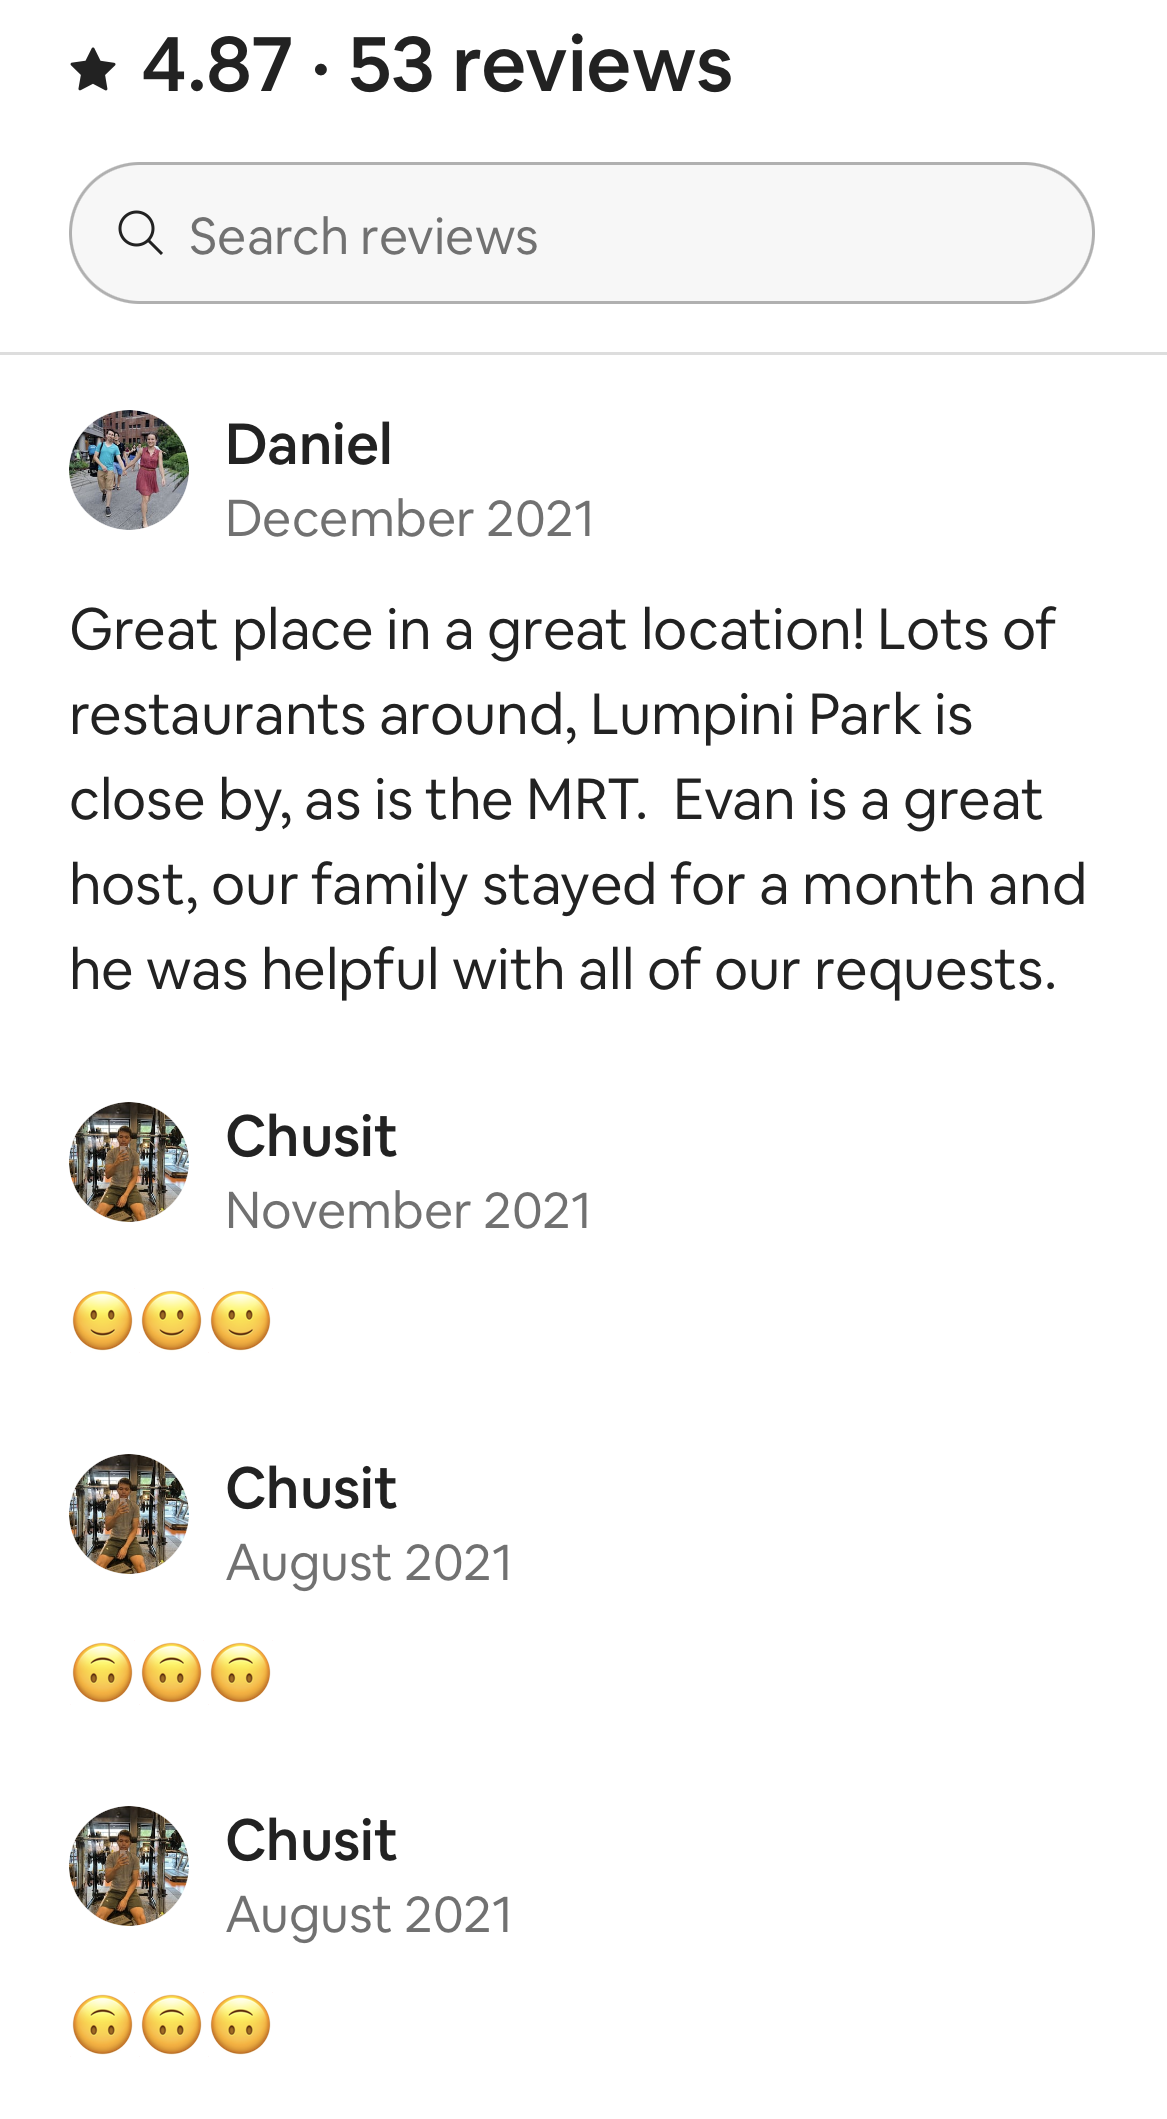
\includegraphics[width=.18\textheight]{query_result_1.png}
		\caption{Reviews from Airbnb app where "listing\_id" = "39539462".}
		\label{fig:015}
	\end{figure}
	\\
	\begin{figure}[h]
		\centering
		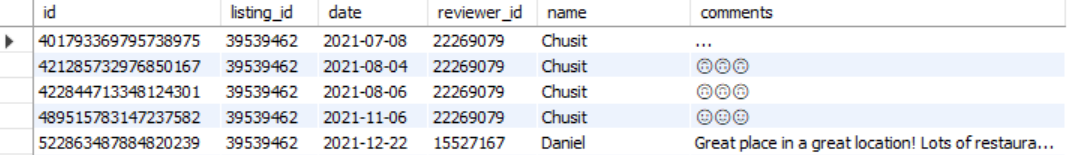
\includegraphics[width=.6\textheight]{sql_result_1.jpg}
		\caption{Reviews from SQL database where "listing\_id" = "39539462".}
		\label{fig:016}
	\end{figure}
	\\
	\begin{figure}[h]
		\centering
		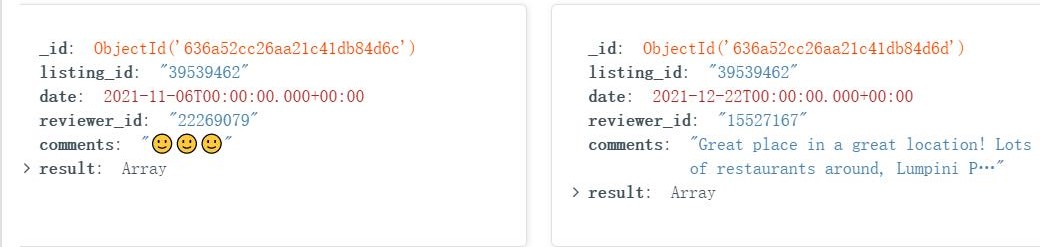
\includegraphics[width=.5\textheight]{query_mongo_1.jpg}
		\caption{Reviews from MongoDB database where "listing\_id" = "39539462".}
		\label{fig:017}
	\end{figure}
	\\
	From the above three results, we can conclude that our databases can perfectly simulate different functions while using Airbnb app. There is no significant difference in response time between two databases; both of them reacts very quickly within a second.  
	\subsection{Comparison between 2 Databases}
	Actually, for these 2 databases, \textbf{each of them has its own edges}. We will briefly discuss as follows:
	\vspace{3pt}
	\\
	\\
	1. \textbf{Schema}. As for \textbf{Relational Database} (Mysql in our report), it has the property that \textbf{RDBMS will try to eliminate Redundancy issues through the storage} if we obey BCNF decomposition. 
	\\
	Moreover, RDBMS can \textbf{better handle Functional Dependency issues}, in the sense that when we need to update with respect to FD, we will have fewer rows to update.
	\\
	As for \textbf{Non-relational Database} (MongoDB in our report), it is totally differenct from RDBMS. It has the adavantage that, the \textbf{schema is more flexible}, which can handle the storage of data stream. 
	\\
	Additionally, \textbf{all the data can be stored in a nested form}, which will bring great benefit to query through join operation (nested can be viewed as join implicitly). Therefore, \textbf{it will make our query requests more efficient}.
	\\
	\\
	2. \textbf{Running Time}
	For the application in Chapter \ref{chapter8.3}, the running time for sql query is  \textbf{0.115} second while for mongoDB query, the running time is  \textbf{0.229} second. We test more cases and find that the running time of two types of queries is short and generally sql query responses a little bit faster. In MongoDB, we \textbf{favor CP, which means we will lose availability}. Therefore, the system may not be able to respond very quickly to the requirements (\textbf{but actually this scenario occurs rarely}).
	\\
	\\
	3. \textbf{Safety}. RDBMS is ACID compliant since we use \textbf{InnoDB} engine, which \textbf{can better handle OLTP}. That is, the whole database system will be safer.
	\vspace{3pt}
	\\
	MongoDB also supports ACID transactions after new version released in 2018, but such function is not applied by default. We do not use this function and whether a database is ACID compliant actually makes no difference in our project. 
	
	
	\section{Workload Description}
	\textbf{Song Mingyue}: mainly focus on EDA and Requirement Analysis;
	\vspace{3pt}
	\\
	\textbf{Yang Sizhe}: mainly focus on Data Cleaning and Data Generation;
	\vspace{3pt}
	\\
	\textbf{Wang Jiangyi}: mainly focus on Relational Database and Report Writing;
	\vspace{3pt}
	\\
	\textbf{Lou Xinyun}: mainly focus on Non-relational Database and Report Writing.
	\section{Summary}
	Lastly, we make a short summary about what we have done in this project:
	\vspace{3pt}
	\\
	1. To \textbf{understand data deeply}, we do Exploration Data Analysis on 3 whole datasets. During this process, we get some insights about the \textbf{data distribution} and figure out the \textbf{data types}. Besides that, we observe something interesting around data, e.g., the \textbf{suspicious review records} (highly likely to be Brushing Fraud Cases). 
	\vspace{3pt}
	\\
	2. To successfully convert 3 datasets into DBMS, we do some data cleaning jobs, especially for the characters in \textbf{text data}. Moreover, we \textbf{do analysis on the null values} and take different actions according to the specific situation.
	\vspace{3pt}
	\\
	3. To enrich our data, we\textbf{ generate transaction records} based on exisiting data. We try our best to make these 'fake' data similar to the real-world data.
	\vspace{3pt}
	\\
	4. We follow the standard pipeline to translate cleaned datasets into relational database and non-relational database. For the \textbf{relational one}, we go step-by-step carefully to \textbf{make sure it is in BCNF}. For the \textbf{non-relation one}, we \textbf{conduct comprehensive schema analysis} to guarantee its performance.
	\vspace{3pt}
	\\
	5. According to the Requirement Analysis of database translation, we give some \textbf{natural language queries} which will \textbf{occur frequently in real-life application}. For the 2 databases, we write the corresponding queries using different database languages. After that, we \textbf{conduct comparison analysis between the 2 databases}.
	
	

\end{document}
